\chapter{The lawn}
\label{ch:lawn}

A real lawn is not a rectangle of cells: it has a curved border, a tree in
the middle, a flower bed, a shed. This chapter describes it as a polygon with
holes, computes its area, decides whether a point is on the lawn, and builds
the fine raster on which the cut grass will be measured.

\section{Polygons with holes}

\begin{definition}{Lawn}{lawn}
  A \emph{lawn} is the region
  \[
    \Omega \;=\; \operatorname{int}(P_0) \setminus
      \bigl(\overline{P_1} \cup \dots \cup \overline{P_k}\bigr)
  \]
  where $P_0$ is a simple polygon (the \emph{border}) and $P_1, \dots, P_k$
  are simple polygons inside it, pairwise disjoint (the \emph{holes}: trees,
  flower beds, buildings). A polygon is given by its vertices
  $p_1, \dots, p_n$, $p_i = (x_i, y_i)$, joined in order and closed
  ($p_{n+1} = p_1$). The mower must cut all of $\Omega$, and its body must
  stay in $\Omega$.
\end{definition}

A curved border is approximated by a polygon with many vertices: the garden
of Figure~\ref{fig:lawns} has 120 vertices on its border and 32 around its
tree.

\begin{figure}[ht]
  \centering
  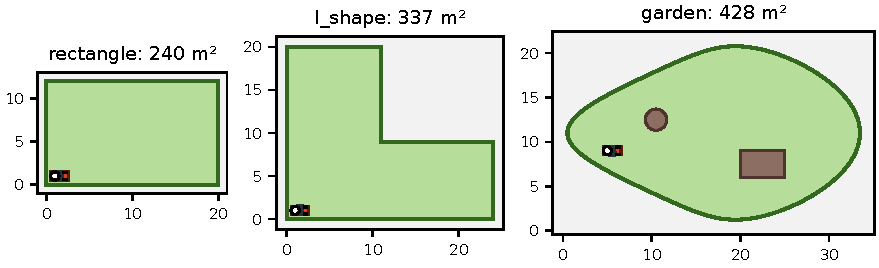
\includegraphics[width=\textwidth]{figures/lawns}
  \caption{The three example lawns of the code (\code{lawns/*.json}),
    in metres. Brown: holes (a round tree and a flower bed in the garden).
    The mower is drawn at its start pose: red body, grey deck with its two
    blade circles, the white dot is the middle of the rear axle.}
  \label{fig:lawns}
\end{figure}

\paragraph{Orientation.}
A polygon is \emph{counter-clockwise} (positively oriented) when the region
it encloses is on the left as one walks along its edges. The code stores the
border counter-clockwise and the holes clockwise, whatever order the file
gives; the next section shows why this convention is convenient.

\section{Area: the shoelace formula}

\begin{proposition}{Shoelace formula}{shoelace}
  The \emph{signed area} of a polygon with vertices $p_1, \dots, p_n$
  ($p_{n+1} = p_1$) is
  \[
    A_s \;=\; \frac12 \sum_{i=1}^{n} \bigl(x_i\,y_{i+1} - x_{i+1}\,y_i\bigr).
  \]
  It equals the area enclosed if the polygon is counter-clockwise, and minus
  the area if it is clockwise.
\end{proposition}

\begin{proof}
  Green's theorem gives the area of a region $D$ whose boundary $\partial D$
  is traversed counter-clockwise:
  \[
    \operatorname{area}(D) \;=\; \frac12 \oint_{\partial D} (x\,dy - y\,dx).
  \]
  The boundary of a polygon is made of the segments $[p_i, p_{i+1}]$.
  Parametrise one of them by
  $p(t) = p_i + t\,(p_{i+1} - p_i)$, $t \in [0, 1]$, and write
  $\Delta x = x_{i+1} - x_i$, $\Delta y = y_{i+1} - y_i$. Then
  $dx = \Delta x\,dt$, $dy = \Delta y\,dt$, and
  \[
    x\,dy - y\,dx
    = \bigl[(x_i + t\Delta x)\,\Delta y - (y_i + t\Delta y)\,\Delta x\bigr]dt
    = (x_i\,\Delta y - y_i\,\Delta x)\,dt,
  \]
  because the terms in $t$ cancel ($t\,\Delta x\,\Delta y -
  t\,\Delta y\,\Delta x = 0$). Integrating over $t \in [0, 1]$:
  \[
    \int_{[p_i, p_{i+1}]} (x\,dy - y\,dx)
    = x_i\,(y_{i+1} - y_i) - y_i\,(x_{i+1} - x_i)
    = x_i\,y_{i+1} - x_{i+1}\,y_i .
  \]
  Summing over the edges and multiplying by $\tfrac12$ gives $A_s$. Walking
  the polygon clockwise reverses every edge, which changes the sign of each
  term.
\end{proof}

\begin{inwords}
  Each edge contributes the signed area of the triangle it forms with the
  origin. Edges seen counter-clockwise from the origin add area, the others
  remove it, and what is left is exactly the inside of the polygon, wherever
  the origin is.
\end{inwords}

\begin{example}{The L-shaped lawn}{lshape}
  The L-shaped lawn of Figure~\ref{fig:lawns} has the vertices
  $(0, 0)$, $(24, 0)$, $(24, 9)$, $(11, 9)$, $(11, 20)$, $(0, 20)$, in metres,
  counter-clockwise. The terms $x_i\,y_{i+1} - x_{i+1}\,y_i$ are, edge by
  edge:
  \begin{align*}
    &0 \cdot 0 - 24 \cdot 0 = 0, &
    &24 \cdot 9 - 24 \cdot 0 = 216, &
    &24 \cdot 9 - 11 \cdot 9 = 117, \\
    &11 \cdot 20 - 11 \cdot 9 = 121, &
    &11 \cdot 20 - 0 \cdot 20 = 220, &
    &0 \cdot 0 - 0 \cdot 20 = 0 .
  \end{align*}
  Their sum is $674$, so the area is $\tfrac12 \times 674 =
  \SI{337}{\metre\squared}$: the $24 \times 9$ rectangle at the bottom
  ($216$) plus the $11 \times 11$ square above it ($121$).
\end{example}

\paragraph{Holes.}
Since the holes are stored clockwise, their signed areas are negative, and the
area to mow is simply the sum of all signed areas:
\[
  A \;=\; A_s(P_0) + A_s(P_1) + \dots + A_s(P_k).
\]

\section{Is a point on the lawn?}

\begin{proposition}{Crossing rule}{crossing}
  Let $P$ be a simple polygon and $q$ a point not on its boundary. Take a
  half-line (a ray) from $q$ that passes through no vertex of $P$. Then $q$ is
  inside $P$ if and only if the ray crosses the edges of $P$ an odd number of
  times.
\end{proposition}

\begin{proof}
  By the Jordan curve theorem, the boundary of $P$ separates the plane into
  two regions, the inside (bounded) and the outside (unbounded). Follow the
  ray from far away towards $q$. Far enough, the ray is outside $P$, since
  $P$ is bounded. Each time it crosses an edge (and not at a vertex), it
  passes from one region to the other; between two crossings it stays in the
  same region. So after an even number of crossings it is outside, and after
  an odd number inside.
\end{proof}

A point is on the lawn if it is inside the border and inside no hole. The
code uses the crossing rule as implemented in Matplotlib
(\code{Path.contains\_points}), applied to the border and to each hole.

\section{The raster}
\label{sec:raster}

Measuring which part of the lawn has been cut means intersecting the lawn
with the area swept by the blades, a shape bounded by thousands of arcs.
Rather than computing with these shapes exactly, the code covers the plane
with small square cells and works cell by cell.

\begin{definition}{Raster}{raster}
  A \emph{raster} of resolution $h$ is a grid of square cells of side $h$. A
  cell is a \emph{lawn cell} if its centre is in $\Omega$. The \emph{raster
  area} of the lawn is $h^2$ times the number of lawn cells.
\end{definition}

The default resolution is $h = \SI{5}{\centi\metre}$: a cell is about the
size of a grass tuft, and the blade circles of Chapter~\ref{ch:mower}, of
radius \SI{25}{\centi\metre}, cover about 80 cells each.

\begin{figure}[ht]
  \centering
  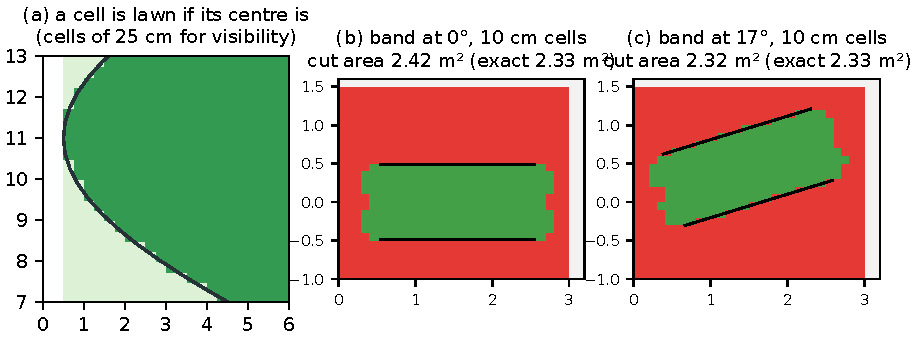
\includegraphics[width=\textwidth]{figures/raster}
  \caption{The raster. (a) The left end of the garden of
    Figure~\ref{fig:lawns} with \SI{25}{\centi\metre} cells (much coarser than
    the \SI{5}{\centi\metre} used in practice, to make them visible): dark
    green cells have their centre on the lawn. (b) and (c) The area cut by a
    \SI{2}{\metre} straight pass of the mower, measured with
    \SI{10}{\centi\metre} cells; black lines: the exact edges of the cut band.
    Green: cut, red: not cut. When the edges run along the grid (b), every
    cell along an edge is wrong in the same direction and the error adds up
    (\SI{2.42}{\metre\squared} measured for \SI{2.33}{\metre\squared}); at
    17° (c), the errors cancel (\SI{2.32}{\metre\squared}).}
  \label{fig:raster}
\end{figure}

\begin{theorem}{Error of the raster area}{rastererror}
  Let the boundary of $\Omega$ (border and holes) be made of $n$ segments of
  total length $\ell$. Then
  \[
    \bigl|A_{\mathrm{raster}} - A\bigr|
    \;\le\; 2\sqrt2\,h\,\ell \;+\; 2\pi\,n\,h^2 .
  \]
\end{theorem}

\begin{proof}
  Write the error as a sum over the cells $c$:
  \[
    A_{\mathrm{raster}} - A
    = \sum_c \Bigl(h^2\,\mathbf 1[\text{centre of } c \in \Omega]
      - \operatorname{area}(c \cap \Omega)\Bigr).
  \]
  A cell that does not meet the boundary of $\Omega$ is entirely inside or
  entirely outside $\Omega$ (it is connected), so its centre is classified
  correctly and its term is $0$. A cell that meets the boundary has a term
  between $-h^2$ and $h^2$. Hence $|A_{\mathrm{raster}} - A|$ is at most $h^2$
  times the number of cells that meet the boundary, that is, at most the
  total area of these cells.

  Each of these cells contains a point of the boundary, and its diameter is
  $\sqrt2\,h$, so all its points are within distance $\varepsilon =
  \sqrt2\,h$ of the boundary. The cells are disjoint, so their total area is
  at most the area of the set $T_\varepsilon$ of points within distance
  $\varepsilon$ of the boundary. For one segment of length $\ell_i$, this set
  is a rectangle $\ell_i \times 2\varepsilon$ with two half-discs of radius
  $\varepsilon$ at its ends, of area $2\varepsilon\,\ell_i +
  \pi\varepsilon^2$. The set $T_\varepsilon$ is the union of these $n$ sets,
  so
  \[
    \operatorname{area}(T_\varepsilon)
    \le \sum_{i=1}^n \bigl(2\varepsilon\,\ell_i + \pi \varepsilon^2\bigr)
    = 2\varepsilon\,\ell + n\pi\varepsilon^2
    = 2\sqrt2\,h\,\ell + 2\pi\,n\,h^2 .
  \]
\end{proof}

\begin{inwords}
  The error comes only from the cells cut by the boundary, so it grows like
  the perimeter times the cell size: halving $h$ halves the bound, while
  quadrupling the number of cells. The bound is a worst case. In practice,
  the cells half in and half out make errors of both signs, which cancel.
\end{inwords}

\begin{example}{The garden}{gardenraster}
  The garden of Figure~\ref{fig:lawns} has $n = 120 + 32 + 4 = 156$ boundary
  segments, of total length $\ell = \SI{104.5}{\metre}$. With
  $h = \SI{0.05}{\metre}$ the bound is
  \[
    2\sqrt2\,h\,\ell + 2\pi\,n\,h^2
    = 2\sqrt2 \times 0.05 \times 104.5 + 2\pi \times 156 \times 0.05^2
    \approx 14.8 + 2.5 = \SI{17.2}{\metre\squared},
  \]
  4\% of its exact area of \SI{427.97}{\metre\squared}. The actual raster area
  is \SI{427.98}{\metre\squared}: an error of \SI{0.01}{\metre\squared}. The
  errors cancel because the border crosses the grid at every angle. A border
  that runs along the grid does not benefit from this cancellation, as
  Figure~\ref{fig:raster}~(b) shows. The code therefore measures the lawn
  and the cut grass on the same raster, so that the coverage ratio compares
  like with like.
\end{example}

\begin{incode}
  \code{mowersim/geometry.py}: \code{Lawn.make(outer, holes)} orients the
  polygons, \code{Lawn.area} is the shoelace formula, \code{Lawn.contains}
  the crossing rule. Lawn files are JSON lists of vertices
  (\code{lawns/garden.json}); \code{tools/make\_lawns.py} writes the
  examples. \code{mowersim/coverage.py}: \code{Raster.of(lawn, res)} builds
  the raster.
\end{incode}
